% Copyright (C)  2015  Alexander Jankowski, Philipp Hacker.
% Permission is granted to copy, distribute and/or modify this document
% under the terms of the GNU Free Documentation License, Version 1.3
% or any later version published by the Free Software Foundation;
% with no Invariant Sections, no Front-Cover Texts, and no Back-Cover Texts.
% The lincense itself can be found at <https://www.gnu.org/licenses/fdl-1.3>.

\documentclass[numbers=noenddot,a4paper]{article}
%\documentclass[numbers=noenddot,12pt,a4paper,notitlepage,twoside,BCOR15mm]{scrartcl}

\usepackage[T1]{fontenc}
\usepackage[utf8]{inputenc}

\usepackage[infoshow]{tabularx}
\usepackage[all]{xy}

\usepackage{amsmath,mathtools}
\usepackage{amssymb}
\usepackage{units}
\usepackage{upgreek}
\usepackage{esint}
\usepackage{graphicx}
\usepackage{ziffer}

\usepackage{float}
\usepackage{lscape}

\usepackage[labelfont=bf]{caption}
\usepackage{wrapfig}
\usepackage{subcaption}

\usepackage[backref=page]{hyperref}

\usepackage{csquotes}
\usepackage[infoshow]{tabularx}
\usepackage{fancyhdr}

\usepackage{sectsty}
\usepackage{times}

\usepackage{lmodern} %TODO Schriftart
\usepackage[greek,ngerman]{babel} %TODO Sprache einstellen

\renewcommand{\headrulewidth}{0.1pt}
\renewcommand{\footrulewidth}{0.1pt}
\newcommand{\name}{\text{Philipp Hacker}} %TODO Name des Protokollanten eintragen

\setlength{\parindent}{0pt}

\newcommand{\degree}{^\circ}
\newcommand{\diff}{\textnormal{d}}
\newcommand{\tenpo}[1]{ 10^{#1}}
\newcommand{\greek}[1]{\greektext#1\latintext}
\newcommand{\ix}[1]{_\text{#1}}
\newcommand{\imag}{\mathbf{i}}
\newcommand{\tilt}[1]{\textit{#1}}
\newcommand{\grad}[1]{\textit{grad}\left(#1\right)}
\newcommand{\divergenz}[1]{\textit{div}\left(#1\right)}
\newcommand{\euler}{\mathnormal{e}}
\newcommand{\fett}[1]{\textbf{#1}}
\newcommand{\ket}[1]{|#1\rangle}
\newcommand{\bra}[1]{\langle#1|}

\title{\fett{\underline{Protokoll: FTIR-Spektroskopie}}} %TODO Name des Versuchs eintragen
\author{Alexander Jankowski, Philipp Hacker}
\date{\today}
\pagestyle{fancy}
\fancyhead[C]{\thepage}
\fancyhead[R]{\name}
\fancyfoot[C]{\thepage}
\fancyhead[L]{Abschnitt \thesection}

\begin{document}

	\renewcommand*{\equationautorefname}{Gl.}
	\renewcommand*{\figureautorefname}{Abb.}
	\renewcommand*{\tableautorefname}{Tab.}
	\renewcommand*{\sectionautorefname}{Abschn.}
	\renewcommand*{\subsectionautorefname}{Abschn.}
	\renewcommand*{\subsubsectionautorefname}{Abschn.}
	\renewcommand*{\figurename}{Abb. }
	\renewcommand*{\tablename}{Tab.}

	\renewcommand*{\figurename}{Abbildung }
	\renewcommand*{\tablename}{Tabelle}


	\maketitle

	\begin{center}
		Betreuer: U. Martens\\ %TODO Name des Betreuers eintragen
		Versuchsdatum: 28.01.2016 \\ %TODO Datum des Versuchs eintragen
		\begin{table}[h]
			\centering
			Note: %TODO Gute Note erhalten :)
			\begin{tabularx}{1.5cm}{|X|}
				\hline \\ \\
				\hline
			\end{tabularx}
		\end{table}
	\end{center}


	\vspace*{\fill}
	\tableofcontents
	\vfill
	\clearpage

	\section{Motivation}

		Eine FTIR-Spektroskopie einer Probe kann dazu genutzt werden, quantitativ als auch qualitativ Informationen \"uber die Zusammensetzung dieser zu erhalten.

	\clearpage
	\section{Physikalische Grundlagen}

		Bei einer FTIR-Untersuchung handelt es sich um die spektroskopische Aufl\"osung von funktionellen Gruppen mit Hilfe der \tilt{Fourier-Transformations-Infra-}\\ \tilt{rotspektrometrie}. Mit einem pr\"azisen Interferometer wird dabei ein Interferogramm - der Verlauf der Interferenzerscheinungen auf dem Schirm des Interferometers, welche durch die \"Uberlagerung von zwei Einzelstrahlen einer IR-Quelle entstehen - aufgenommen, welches dann \"uber eine \tilt{Fourier-Transformation} aus dem Orts- in den Frequenzraum abgebildet wird.\\
		Die bei der FTIR-Spektroskopie benutzte Infrarotstrahlung im Wellenl\"angenbereich zwischen $\unit[[2500-15400]]{nm}$ bzw. den Wellenzahlen $\unit[[4000-650]]{cm^{-1}}$ regt in der, im Strahlengang des Interferometers befindlichen Probe, Molek\"ulschwingungen an. Verschiedene Arten von Molek\"ulen bzw. funktionellen Gruppen dieser, welche wiederum anders in der Probe gebunden sind, haben unterschiedliche Eigenfrequenzen der Schwingungen. Durch diese Anrgegung wird Energie aus der elektromagnischen Welle von der Probe absorbiert, was ein, f\"ur das zu untersuchende Objekt spezifisches Absorptionsspektrum liefert. Der Teil der Welle, welcher nicht absorbiert, sondern einfach transmittiert wird, ergibt wiederum ein einzigartiges Transmissionsspektrum. Diese \tilt{Fingerabdruck-Methode} bedarf einer umfangreichen Datenbank von Korrelationstabellen - Literaturspektren zu bekannten Materialien/Proben - um das eigene Spektrum einordnen und schlie{\ss}lich eine Bestimmung der Molek\"ul(-gruppen) vornehmen zu k\"onnen.\\
		Das quantenmechanische Modell bedient sich der parabolischen N\"aherung des harmonischen Potentialminimums der Molek\"ulbindungen. Man geht dabei au{\ss}erdem davon aus, dass die Relativbewegung von Atomkernen und Elektronen von den wesentlich schnelleren und leichteren Fermionen bestimmt wird - die tilt{Born-Oppenheimer-N\"aherung}. Des weiteren erh\"alt man aus solchen Schwingungen nur Infrarotstrahlung, wenn ein vorliegendes Dipolmoment sich zeitlich \"andert. Die station\"are Schr\"odingergleichung f\"ur ein Molek\"ul\ im Zustand $\Psi(\vec{x})$ mit den Atomen der reduzierten Massen $\mu$	lautet folglich \cite{FTIRInfra}
		
			\begin{align}
				-\frac{\hbar^{2}}{2\mu}\frac{\diff^{2}\Psi(\vec{x})}{\diff x^{2}}+V(\vec{x})\Psi(\vec{x})=E\Psi(\vec{x}) \label{eq:schroed}
			\end{align}
	
		F\"ur das Potential $V(\vec{x})=k/2\cdot (\vec{x}-\vec{x}\ix{0})^{2}$ um die Gleichgewichtslage $\vec{x}\ix{0}$ liefert \autoref{eq:schroed} das Ergebnis f\"ur die Energiesniveaus $E_{\nu}$ nach den Schwindungsquantenzahlen $\nu$:
	
			\begin{align}
			\Aboxed{E_{\nu}=(\nu+\frac{1}{2})\cdot\hbar\sqrt{\frac{k}{\mu}}.} \label{eq:energie}
			\end{align}
	
		F\"ur die Vereinfachung, dass die Molek\"ule n\"aherungsweise harmonische Oszillatoren sind (s.o.), so gilt die Auswahlregel f\"ur \"Uberg\"ange in dem erzeugten Schwingungspektrum $\Delta\nu=\pm1$. Die Absorption von einem Photon der Energie $\hbar\omega=\hbar\sqrt{k/m}$ entspricht demnach dem \"Ubergang von $\nu\rightarrow\nu+1$.\\
		Starke chemische Bindungen von Atomen kleiner Massen ben\"otigen gro{\ss}e Schwingungsquanten, schw\"achere Bindungen schwerer Atome kleinere.\\
		Unterschieden werden muss im IR-Spektrum noch zus\"atzlich die Art der Molek\"ulschwingung: Normalschwingungen erzeugen nicht immer Infrarotstrahlung, sondern nur dann, wenn sich innerhalb des System des Molek\"uls L\"angen oder Winkel \"andern. Demnach geh\"oren bspw. Translationen und Rotationen nicht zu den IR-aktiven Schwingungen.
	
	\subsection*{Interferometrie und Fourier-Transformation}
	
		Das Interferometer innerhalb des Spektrometers besteht aus einem halbdurchl\"assigen Strahlteiler, einem festen sowie einem beweglichen Spiegel. Die normale Infrarotstrahlung eines - im Idealfall - erhitzten \tilt{schwarzen K\"orpers} \cite{FTIRSpek} mit Wellenzahlen $\unit[[400-7800]]{cm^{-1}}$ (Infrarot $\leftrightarrow$ W\"armestrahlung) wird an dem Strahlteiler aus Kaliumbromid - Transmission bei $\unit[[400-7800]]{cm^{-1}}$ - in zwei Teilstrahlen aufgeteilt. Wie in einem \tilt{Michelson-Interferometer} werden diese dann einerseits auf den feststehende, andererseits auf den beweglichen Spiegel gelenkt. Auf dem selben Strahlteiler kommt es danach zu verschiedenen Interferenzerscheinungen zwischen den reflektierten Strahlen, je nachdem, welche optische Wegdifferenz und Frequenz vorliegt.\\
		Der wieder zusammengef\"uhrte Strahl wird durch eine Blende, den \tilt{J-Stopp}, auf die Probe geleitet. Dort werden die Molek\"ulschwingungen von der Infrarotstrahlung angeregt, woraus die charakteristische Absorption bzw. Transmission in Abh\"angigkeit der Frequenz folgt. Ein \tilt{DTGS}-Detektor - kristallines \tilt{Deuteriertes Triglycinsulfat} hat die g\"unstige pyroelektrische Eigenschaft, das Ladungstrennung bei Temperatur\"anderungen/Verformungen aufgrund polarer Einheitszellen eintritt - nimmt das erhaltene Signal in Abh\"angigkeit der Stellung des beweglichen Spiegels auf. Dieses nicht-korrigierte Interferogramm als Funktion $I\ix{IF}(x)$ von der optischen Wegdifferenz $x$ muss noch um einen konstanten Teil - Beachtung des, an die Quelle verloren gegangenen reflektierten Teils - berichtigt werden. Schlie{\ss}lich erh\"alt man aus einer  \tilt{Cosinus-Fourier-Transformation} aus dem Orts- in den Frequenzraum das Spektrum $I\ix{F}(f)$,
		
			\begin{align}
			\Aboxed{
				I\ix{F}(f)=\int_{-\infty}^{+\infty}I\ix{IF}(x)\cdot\cos(2\pi\nu^{\prime}x)\diff \nu^{\prime}.
				} \label{eq:fourier}
			\end{align}
		
		Im allgemeinen gibt man das Spektrum in Abh\"angigkeit von der Wellenzahl $k=2\pi/\lambda$ an. Demnach findet man die Absorptionsbanden von \tilt{Streckschwingungen} der Molek\"ule des Typs \tilt{X-H}, wobei \tilt{X} ein beliebiges Atom und \tilt{H} Wasserstoff ist, im Bereich von $\unit[[2500-4000]]{cm^{-1}}$. Die st\"arkeren 3-fach Bindungen findet man hingegen im Bereich $\unit[[2000-2500]]{cm^{-1}}$ auf Grund ihrer h\"oheren Kopplungskonstante des Bindungspotentials. Au{\ss}erdem k\"onnen zu diesem Spektralbereich auch X-H-Streckschwingungen mit schweren X-Atomen beitragen. Der Gr\"o{\ss}te Anteil im Bereich zwischen $\unit[[1500-2000]]{cm^{-1}}$ ist den Streckschwingungen der Doppelbindungen mit Kohlenstoffatomen zu zuordnen \cite{FTIRAns}.\\
		Im sogenannten ``Fingerprint''-Bereich zwischen $\unit[[400-1500]]{cm^{-1}}$ manifestieren sich vor allem feinste Unterschiede zwischen \"ahnlichen Molek\"ulen, welche durch chemische unterschiedliche Anbindungen, die Umgebung oder Defekte hervorgerunfen werden. Solche sind s\"amtliche elektronischen Effekte sowie Beuge- und Ger\"ustschwingungen.\\
		Schlie{\ss}lich gilt es zu beachten, dass nat\"urlich auch die Wechselwirkung induzierter/permanenter Dipole in der Probe mit der Infrarotstrahlung eine Ver\"anderung des reinen Schwingungsspektrums hervor ruft.
		
	\clearpage
	\section{Durchführung}



	\clearpage
	\section{Auswertung}

%	\begin{figure}
%		\includegraphics[width=\textwidth]{Gruppe2A/inter.pdf}
%		\caption{Interferogramm}
%		\label{img:inter}
%	\end{figure}
%	
%	\begin{figure}
%		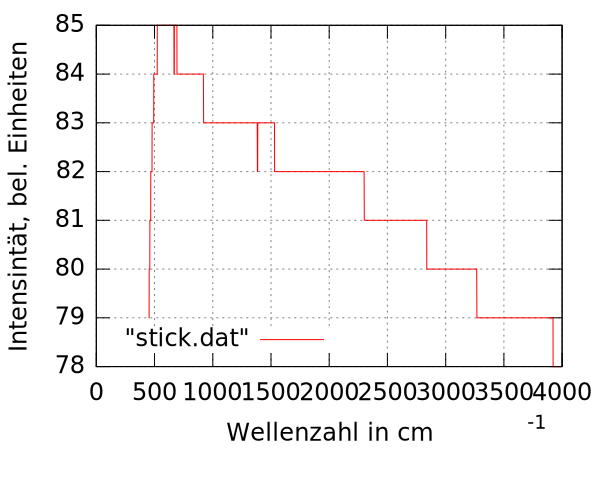
\includegraphics[width=\textwidth]{Gruppe2A/stick.pdf}
%		\caption{}
%		\label{img:stick}
%	\end{figure}
%	
%	\begin{figure}
%		\includegraphics[width=\textwidth]{Gruppe2A/meth.pdf}
%		\caption{}
%		\label{img:meth}
%	\end{figure}
%
%	\begin{figure}
%		\includegraphics[width=\textwidth]{Gruppe2A/meth_diff.pdf}
%		\caption{}
%		\label{img:meth_diff}
%	\end{figure}
	
	\clearpage
	\section{Anhang}

		\bibliography{all.bib}
		\bibliographystyle{unsrt}

\end{document}